The \textit{Lomb-Scargle} method of PSD-estimation can be classified as a method of ``Least-squares spectral analysis'' (LSSA). LSSA tries to extend the periodogram estimation to data sequences that are not necessarily sampled in an equally-spaced manner. This also applies if individual samples of the data are lost or could not be aquired and will remove the need to resample or interpolate the data. \cite{lomb_1}\cite{yt_video}\\

Instead of explicitly performing the Fourier transform, the Lomb-Scargle periodogram estimates the PSD using a sinusoidal model that matches the data. The Lomb-Scargle technique looks for the model that best explains the data as a sum of sinusoids with various frequencies and amplitudes.

The algorithm first determines a range of frequencies for measuring the PSD. These frequencies, which might be evenly or logarithmically separated, are determined by the frequency range anticipated in the signal. The program then uses a weighted sum of the data points, where the weights vary depending on how well the model fits the data, to compute a power estimate at each frequency.

Least-squares fitting is employed to determine the weights. In order to achieve this, one must identify the set of parameters that minimizes the total of the squared discrepancies between the model and the data at each moment. These weights are then used by the algorithm to determine the power estimate for each frequency.

However, the method has significant drawbacks. It's assumption that the signal is stationary, which may not be the case for all signal types, is one of its limitations. The method may also be sensitive to the selection of model parameters, such as the quantity of frequencies employed in the model or the frequency range assessed. \cite{saqib_1}\cite{saqib_2}\cite{saqib_3}\\

To simulate this method, signal $A$ was sampled at uniformly distributed random times. As seen in Figure \ref{fig:lomb_1}, the Lomb-Scargle periodogram approximately follows the standard periodogram.


\begin{figure}[H]
\centering
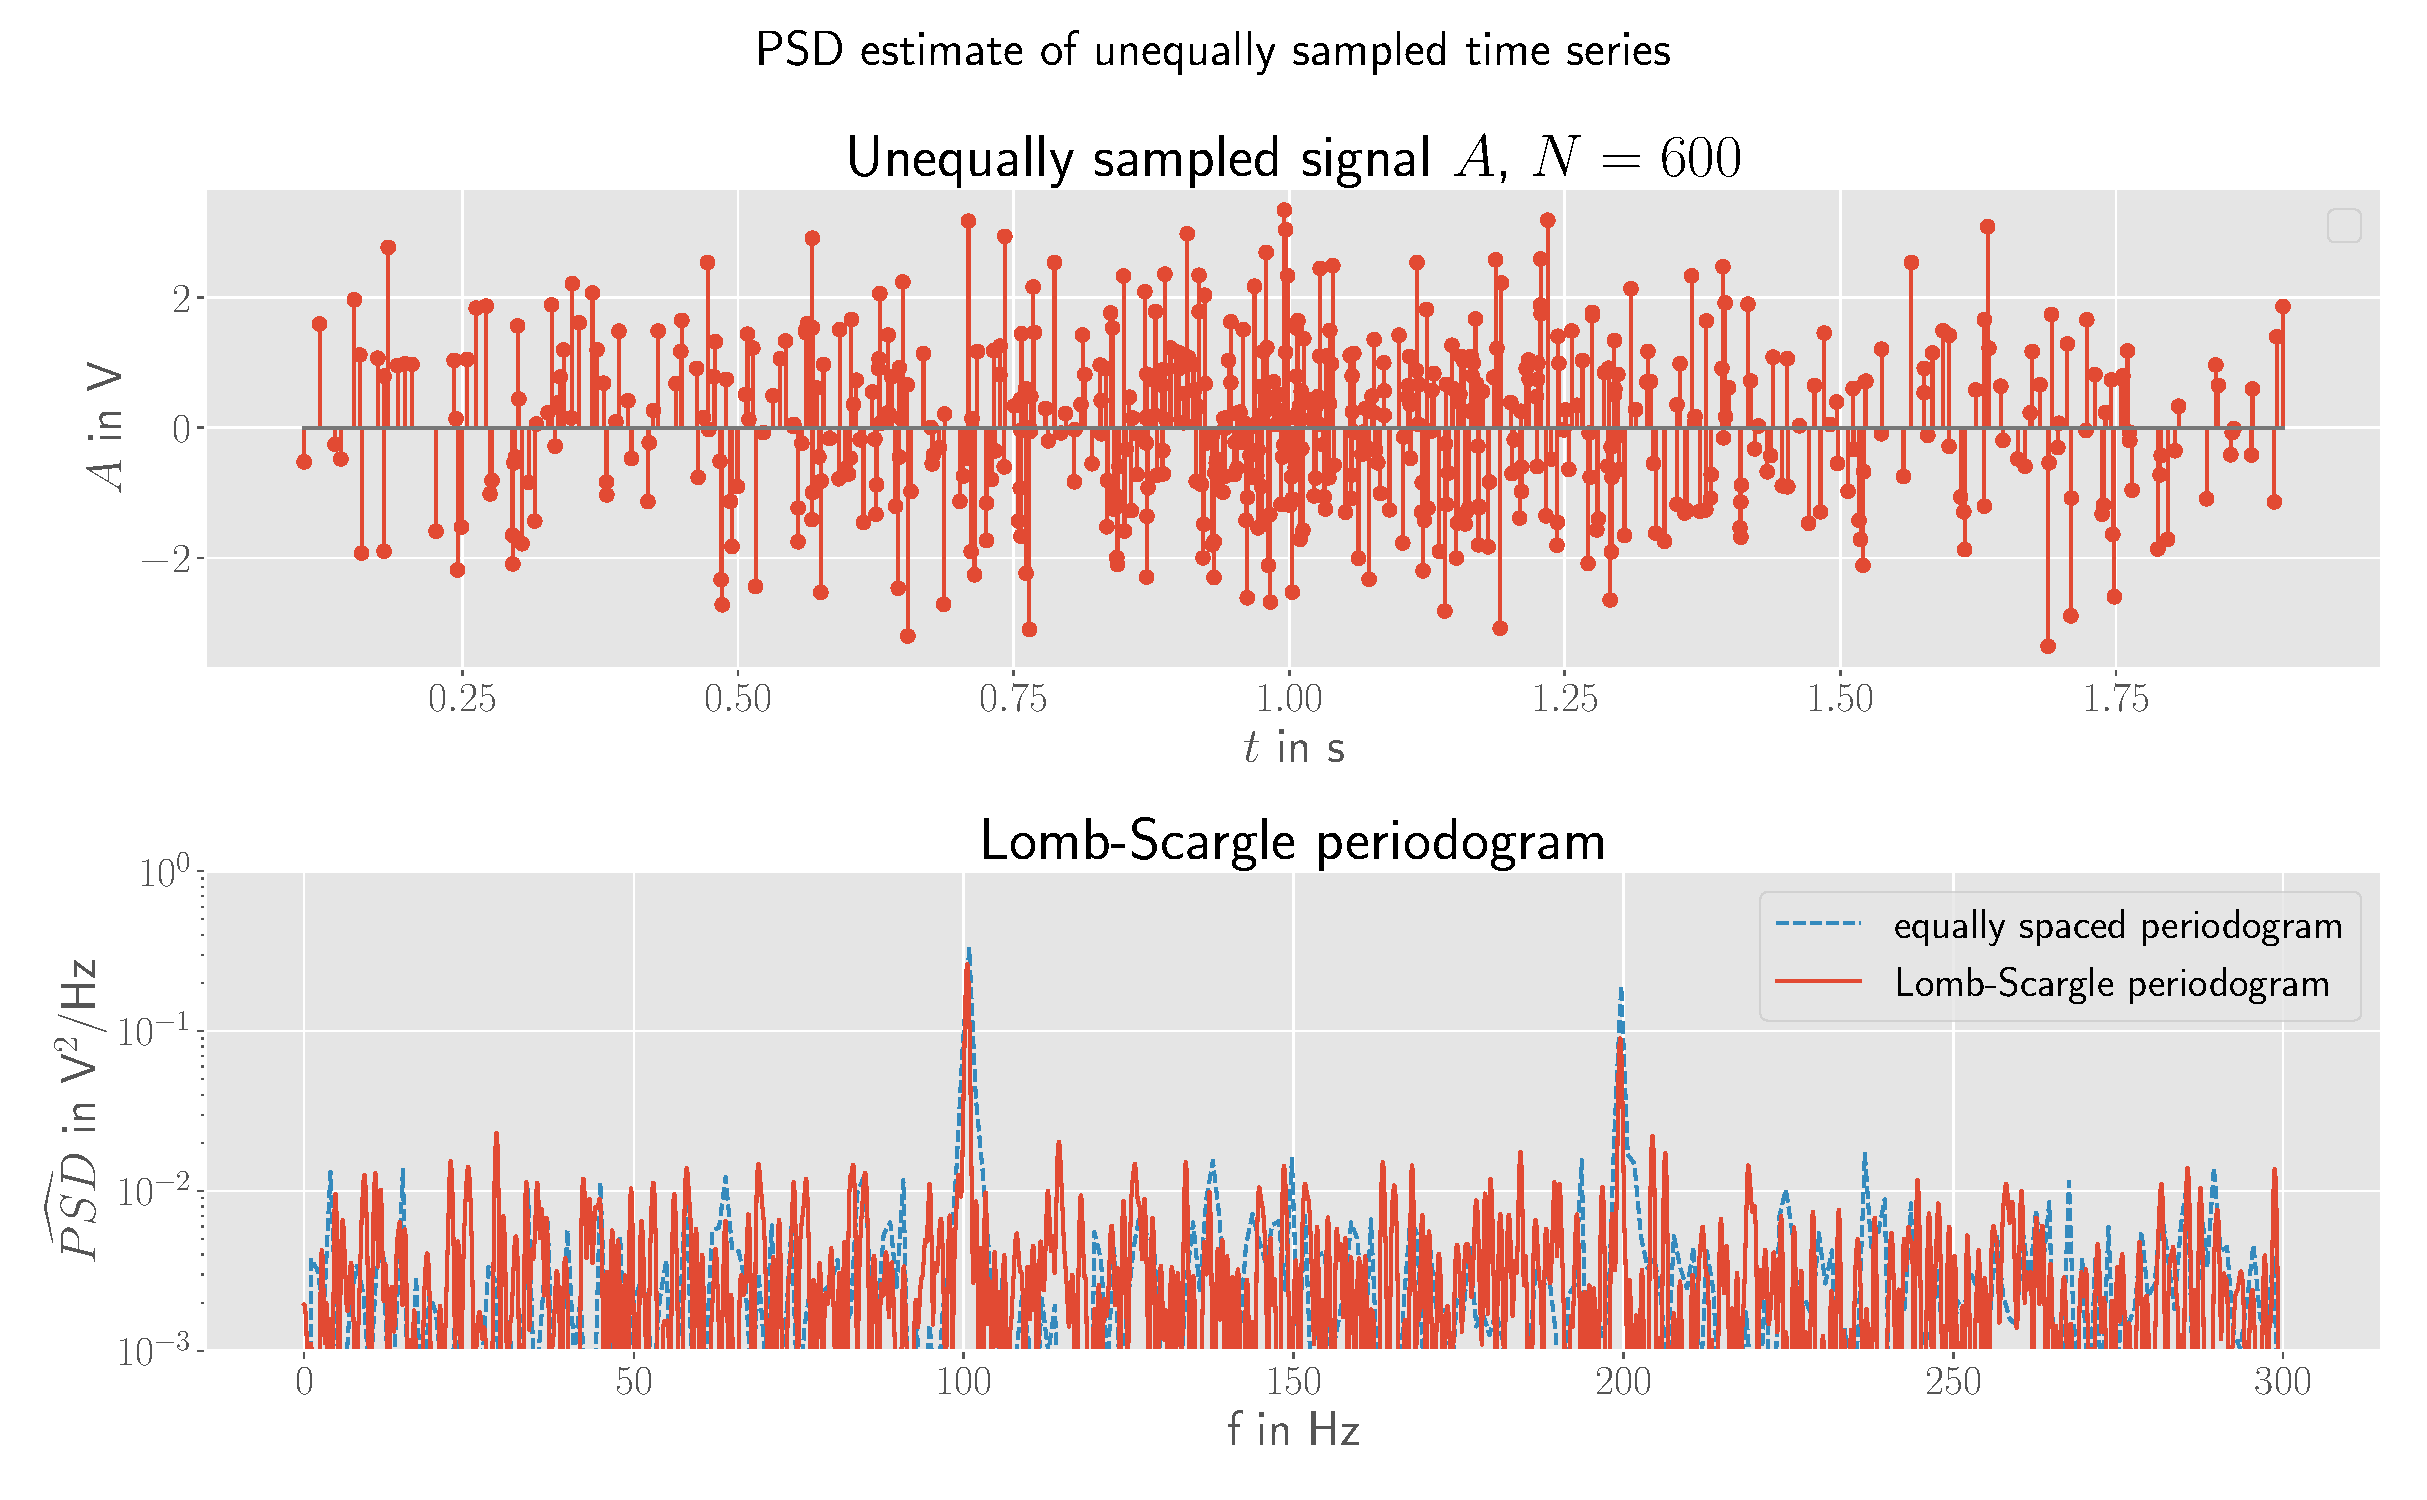
\includegraphics[width=0.764\textwidth]{graphics/lomb_scargle.pdf}
\caption{Lomb-Scargle PSD estimate of an unevenly spaced }\label{fig:lomb_1}
\end{figure}

